\documentclass{article}

\usepackage[utf8]{inputenc}
\usepackage[russian]{babel}
\usepackage[a4paper, margin=1in]{geometry}
\usepackage{graphicx}
\usepackage{amsmath}
\usepackage{wrapfig}
\usepackage{multirow}
\usepackage{mathtools}
\usepackage{pgfplots}
\usepackage{pgfplotstable}
\usepackage{setspace}
\usepackage{changepage}
\usepackage{caption}
\usepackage{csquotes}
\usepackage{hyperref}
\usepackage{listings}

\pgfplotsset{compat=1.18}
\hypersetup{
  colorlinks = true,
  linkcolor  = blue,
  filecolor  = magenta,      
  urlcolor   = darkgray,
  pdftitle   = {
    database-report-1-smirnov-victor-p33131
  },
}

\definecolor{codegreen}{rgb}{0,0.6,0}
\definecolor{codegray}{rgb}{0.5,0.5,0.5}
\definecolor{codepurple}{rgb}{0.58,0,0.82}
\definecolor{backcolour}{rgb}{0.99,0.99,0.99}

\lstdefinestyle{codestyle}{
  backgroundcolor=\color{backcolour},   
  commentstyle=\color{codegreen},
  keywordstyle=\color{magenta},
  numberstyle=\tiny\color{codegray},
  stringstyle=\color{codepurple},
  basicstyle=\ttfamily\footnotesize,
  breakatwhitespace=false,         
  breaklines=true,                 
  captionpos=b,                    
  keepspaces=true,                 
  numbers=left,                    
  numbersep=5pt,                  
  showspaces=false,                
  showstringspaces=false,
  showtabs=false,                  
  tabsize=2
}

\graphicspath{ {./img/} }

\lstset{style=codestyle}

\begin{document}

\begin{titlepage}
    \begin{center}
        \begin{spacing}{1.4}
            \large{Университет ИТМО} \\
            \large{Факультет программной инженерии и компьютерной техники} \\
        \end{spacing}
        \vfill
        \textbf{
            \huge{Базы данных.} \\
            \huge{Лабораторная работа №2.} \\
        }
    \end{center}
    \vfill
    \begin{center}
        \begin{tabular}{r l}
            Группа:  & P33131                  \\
            Студент: & Смирнов Виктор Игоревич \\
            Вариант: & 310963
        \end{tabular}
    \end{center}
    \vfill
    \begin{center}
        \begin{large}
            2023
        \end{large}
    \end{center}
\end{titlepage}

\section*{Ключевые слова}

База данных, нормальная форма.

\tableofcontents

\section{Цель работы}

Изучить методы нормализации баз данных.
Проанализировать свою схему на 
соответствие нормальным формам.

\section{Функциональные зависимости}

\begin{figure}[th]
  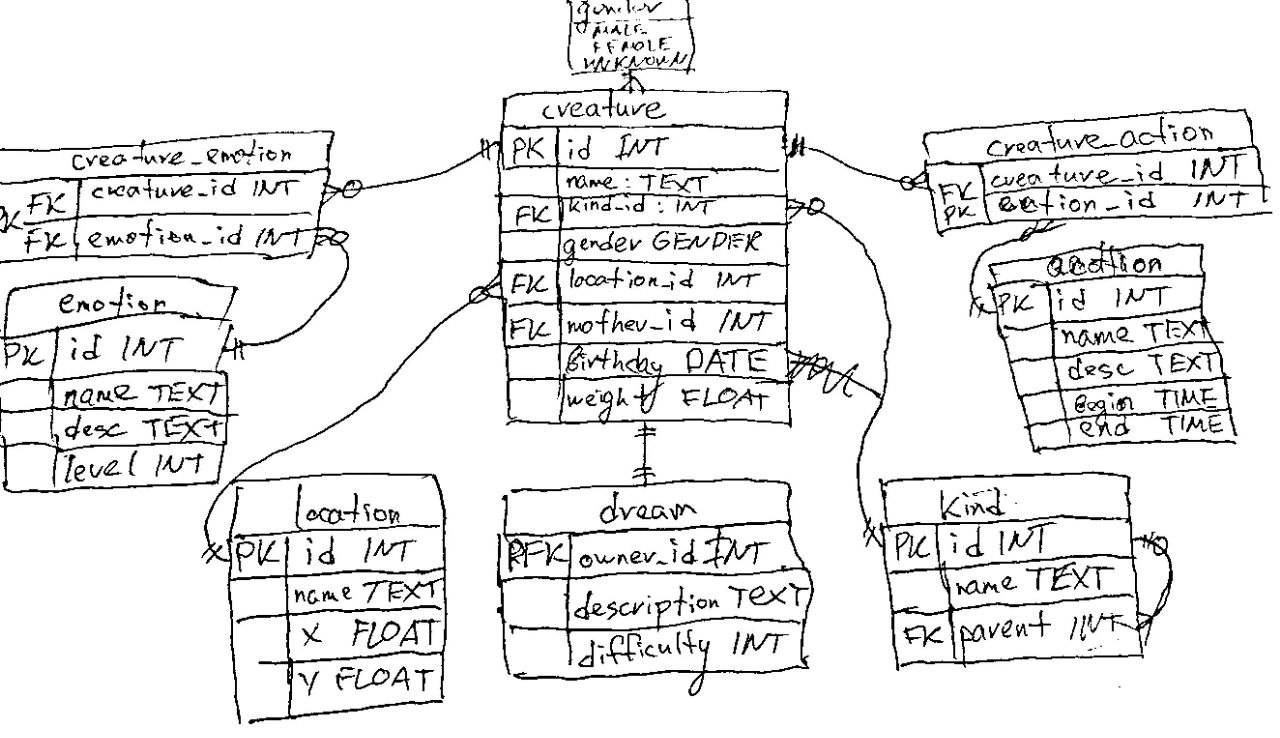
\includegraphics[scale=0.2]{../lab-1/fig/er.jpg}
  \centering
\end{figure}

\begin{lstlisting}
creature:
  id -> name
  id -> kind_id
  id -> gender
  id -> location_id
  id -> mother_id
  id -> birthday
  id -> weight

  mother_id -> kind_id ?

emotion:
  id -> name
  id -> desc
  id -> level

location:
  id -> name
  id -> x
  id -> y

dream:
  owner_id -> description
  owner_id -> difficulty

kind:
  id -> name
  id -> parent

emotion:
  id -> name
  id -> description
  id -> begin
  id -> duration
\end{lstlisting}

\section{1 НФ}
Ни один кортеж не содержит в
каждом поле более одного
значения.

\section{2 НФ}

Все поля, не входящие в
первичный ключ находятся
в полной функциональной
зависимости от ПК.

\section{3 НФ}

Нет транзитивных зависимостей.

\section{БКНФ}

Любая функциональная
зависимость между полями
сводиться к полной
функциональной зависимости от
ключа, т.е. в составном
ключе все эл-ты независимы.

\section{Денормализация}

Можно слить таблицы emotion и creature\_emotion.
Или анологично поступить с action. Тогда 
придется дублировать данные одной и той же эмоции,
что приведет к тому, что одно изменение будет 
распостронятся сразу же на несколько строк.
Тогда нарушится 2 НФ, так как данные будут зависеть
лишь от части ПК -- идентификатора эмоции.

Можно влить те же эмоции в таблицу
с существами, но тогда вообще не будет и 
1 НФ.

\section{Вывод}

Нормализация баз -- формальный метод рефакторинга 
баз данных с целью упрощения базы данных, 
повышения расширяемости и улучшения согласованности
данных. Мне этот метод показался трудно применимым
на практике, ведь чаще всего просто чувство 
разработчика о том, что есть хорошо, а что есть
плохо, с меньшими потерями позволяет улучшить БД.
С другой стороны, такие правила могут лечь в 
основу алгоритмов статических проверок качества 
схемы БД. Нормализация таблицы,
кажется, часто ведет к
более простая, элегнатная,
более single-responsible.
Процесс нормализации таблицы
может помочь для рефакторинга
плохо спроектированных БД.
Но не всегда делают лучше,
а еще влияют на
производительность.

% \begin{thebibliography}{9}
    
% \end{thebibliography}

\end{document}